\documentclass[a4paper, 14pt]{report}

\usepackage{cmap}
\usepackage[T2A]{fontenc}
\usepackage[utf8]{inputenc}
\usepackage[english,russian]{babel}
\usepackage[left=30mm, top=20mm, right=20mm, bottom=20mm, nohead, nofoot]{geometry}
\usepackage{indentfirst}

\usepackage{amsmath}
\usepackage{MnSymbol}
\usepackage{wasysym}

\usepackage{graphicx}
\graphicspath{{img/}}
\DeclareGraphicsExtensions{.pdf}

\usepackage{pgfplots}
\pgfplotsset{compat=1.16}

\usepackage{listings}

\lstset{
    numbers=left,
    frame=single,
    texcl=true,
    basicstyle=\ttfamily,
    mathescape
}

\author{Ульянов Михаил Васильевич}
\title{Анализ алгоритмов}
\date{2019}

\begin{document}
\maketitle

\tableofcontents
\clearpage

\chapter{Исторический очерк}

\begin{enumerate}
    \item \textbf{1900} \newline
        Д. Гильберт - 23 проблемы
        1931 - К. Гедель доказал теорему о неполноте
    \item \textbf{1936} \newline
        А.Тьюринг, Э.Л.Пост - Теория алгоритмов (начало)
    \begin{enumerate}
        \item[-] формализация понятия
        \item[-] общие свойства
        \item[-] обнаружение алгоритмически неразрешимых задач
    \end{enumerate}
    \item \textbf{1960е} \newline
        Теория сложности вычислений NPC \newline
        $O(n^2)\ O(n \cdot \ln(n))$

        \begin{tikzpicture}
            \begin{axis}[
                xlabel = {$n$},
                minor tick num = 10,
                domain=0:10,
                legend pos = north west,
                grid = major,
                line width = 1
            ]
                \legend{
                    $n^2$,
                    $n \cdot \ln(n)$
                };

                \addplot[blue] {x^2};
                \addplot[orange] {3 + x*ln(x)};
            \end{axis}
        \end{tikzpicture}

    \item \textbf{Начало 1970х} \newline
        Практический анализ алгоритмов Д.Э. Кнут
\end{enumerate}

\chapter{Схема выбора алгоритмического обеспечения}

Нет:

\begin{enumerate}
    \item[A.] Новый (метод разработки)
    \item[B.] Комбинированные элементы ($A_1 + A_2 + A_3$)
\end{enumerate}

$$ Q(q_1,...,q_m) = \sum \alpha_i q_i \to R^1 \text{ - комплексные оценки}$$

$$
\begin{cases}
    a_{11} x_1 + a_{12} x_2 = b_1 \\
    a_{21} x_1 + a_{22} x_2 = b_2
\end{cases}
$$

$$ a + ib = (c + id) = ^{det} (ac - bd) + i (bc + ad) $$

\chapter{1936 год Э.Л. Пост "Финитные комбинаторные процессы - формулировка 1"}

\section{Терминология}

Общая проблема = задача

Конкретная проблема = индивидуальная задача

\section{Общая проблема}

Общая $\to$ множество всех конкретных

Решение общей $\to$ решение каждой конкретной

\section{Пространство символов}

\begin{tabular}{c|c|c|c|c|c|c|c}
    \hline
    $\leftarrow$ & & & & & & & $\to$ \\
    \hline
\end{tabular}

\hfill

\begin{tabular}{c|c|c}
    \hline
    & Помечен, не помечен & \\
    \hline
\end{tabular}

\hfill

Конкретная проблема задается внешней силой путем пометки конечного числа символов.

\section{Работник (процессор)}

\begin{enumerate}
    \item $\to$  (R)
    \item $\leftarrow$ (L)
    \item $\checkmark$ Поставить метку, если пусто
    \item $\xi$ Стереть, если есть
    \item ? $\begin{matrix}
            \overset{\text{да}}{\to} N^o \text{ строки} \\
            \overset{\text{нет}}{\to} N^o \text{ строки} \\
            \end{matrix}$
    \item stop
\end{enumerate}

\section{Примеры}

\begin{tabular}{c|c|c|c|c|c|c|c}
    \hline
    & $\checkmark$ & $\checkmark$ & $\checkmark$ & $\checkmark$ & ... & $\checkmark$ &  \\
    \hline
\end{tabular}

\begin{enumerate}
    \item $\xi$
    \item $\to$
    \item ? $\begin{matrix}
            \overset{\text{да}}{\to} 1 \\
            \overset{\text{нет}}{\to} 4 \\
            \end{matrix}$
    \item stop
\end{enumerate}

\section{Гипотеза Поста}

\begin{enumerate}
    \item[a)] Программа применима к общей, если $\forall$ конкретной нет коллизий в операциях 3,4
    \item[b)] программа заканчивается, если stop
    \item[c)] Если $\forall$ конкретной внеш сила распознает правильный ответ, то Ф1П есть 1-решение общей
    \item[d)] Мы вправе рассматривать все более и более широкие формулы

        $$
            \begin{array}{l}
            \text{пространство символов} \\
            \text{алфавита} \\
            \text{набор инструкций} \\
            \end{array}
        \text{логически сводимы к формуле 1}
        $$
\end{enumerate}

a + b = Финитный 1 процесс

\section{1984 Муравей Лэнгтона}
\begin{tabular}{c|c|c|c|c|c|c}
    & & & & & & \\
    \hline
    & & $\blacksquare$ & $\blacksquare$ & & & \\
    \hline
    & & $\blacksquare$ & & $\blacksquare$ & & \\
    \hline
    & & & $\blacksquare$ & $\blacksquare$ & & \\
    \hline
    & & & & & & \\
\end{tabular}

$$
W \to (B,R)
$$

$$
B \to (W,L)
$$

%
%
%
%
%
%
%
% ПРОПУСК У АРТУРА
%
%
%
%
%
%

\chapter{Терминология}

\section{Вход алгоритма}

Конкретная проблема $\Rightarrow$ индивидуальная задача $\Rightarrow$ Вход
$D = \{ d_i | i = 1,m \}$

\section{Длина входа}

$n \to |D| ?$

$$
\mu_z (D) \to g(|D|)
$$

$$
\mu_{sort} (D) = |D| - 1
$$

Умножение матриц $n \times n$

$$
|D| = 2n^2 + 1
$$

$$
\mu_z(D) = n = \sqrt{\frac{|D| - 1}{2}}
$$

\section{Трудоемкость}

$f_A(D)$ - число элементарных операций принятой модели вычислений заданных
алгоритмом $A$ на входе $D$

$$
f_{A_1} (D) < F_{A_2} (D)
$$

\section{$D_n$}

$$
D_n = \{ D | \mu_z(D) = n \}
$$

$$
\beta = 16\ \ |D_{10}| = 2^{160}
$$

\section{Переход к n}

$$
f_A^\vee(n) \overset{def}{=} \underset{D \in D_n}{min} f_A(D) \text{ - лучший случай}
$$

$$
f_A^\wedge(n) \overset{def}{=} \underset{D \in D_m}{max} f_A(D) \text{ - худший случай}
$$

$$
\overline{f}_A(n) = \sum_{D \in D_n} p(D) - f_A(D)
$$

$$
p(D) = \frac{1}{|D_n}
$$

\section{Память}

$$
V(D) = \underset{\text{Вход}}{|D|} + \underset{\text{Результат}}{|R|} + V_\text{допольнительно памяти}(D) + V_\text{программы}
$$

$$
V_A(D) = V_\text{доп}(D) | V^\vee(n), V^\vee(n), ...
$$

\chapter{Примеры}

\section{Умножение матриц}

\begin{lstlisting}
MultM(A,B,n;C)
    for i $\leftarrow$ 1 to n
        for j $\leftarrow$ 1 to n
            s $\leftarrow$ 0
            for k $\leftarrow$ 1 to n
                s $\leftarrow$ s + A[i,k] * B[k,j]
            c[i,j] $\leftarrow$ s
End
\end{lstlisting}

$$
f^\vee_A(n) = f^\wedge_A(n)=f_A(n) = 1 + n (3 + 1 + n (3 + 2 + n (3 + 7) + 3)) =
10 n^3 + 8n^2 + 4n + 1
$$

\section{Max}

\begin{lstlisting}
Max(A,n;M)
    M $\leftarrow$ A[1]
    for j $\leftarrow$ 2 to n
        if M < A[i]
            M $\leftarrow$ A[i]
End
\end{lstlisting}

$$
f^\vee_A(n) = 2 + 1 + (n-1) (3+2) = 5n - 2
$$

$$
f^\wedge_A(n) = 2 + 1 + (n_1) (3+2+2) = 7n - 4
$$

\section{Степень}

\begin{lstlisting}
Pow(x,k;y)
    ...
    y $\to$ 1
    for j $\to$ 1 to k
        y $\to$ y * x
End
\end{lstlisting}

$$
D \in D_2
$$

$$
M_z(D) = 2
$$

$$
f_A(k) = 2 + 5k
$$

$$
e^x=e^{\lfloor x \rfloor} \cdot e^{\{x\}}
$$

$$
e^\alpha = \sum^\infty \frac{\alpha^k}{k!}, 0 \le \alpha < 1,
\frac{\alpha^k}{k!} > \sum_{k+1}^\infty (.)
$$

$$
\text{Exp}(x,eps,y) \Rightarrow k^* = g(eps)\ \ k^* : \frac{\alpha^{k^*}}{k^*!}
$$

\chapter{Классификация алгоритмов по типу трудоемкости}

\section{Класс N - количесвенно-зависимые алгоритмы}

$$
f_A(D) = f_A(\mu_Z(D)) = f_A (n)
$$

$$
f^\vee = f^\wedge!
$$

!Матрично-векторные операции

\begin{center}
    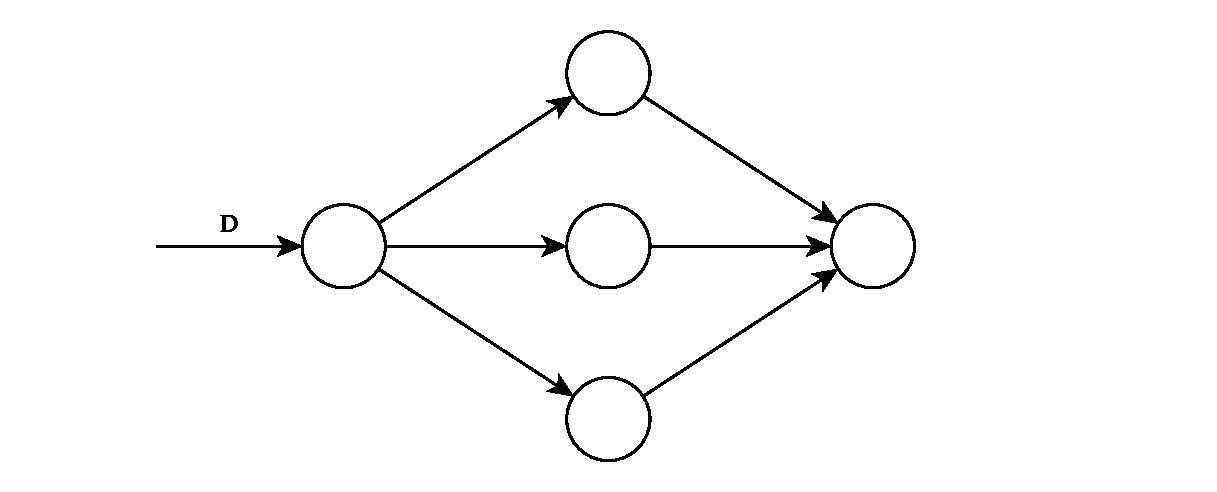
\includegraphics[scale=0.5]{anal1}
\end{center}

Гипотеза П.Леви

$$
R^n\ \overline{a} = (..., [-1,1], ...)
$$

\section{Класс PR - параметрически-зависимые алгоритмы}

$$
f_A(D) = f_A(P+1,...,p+k) \ne f(n)
$$

$$
li(x0) = \int_2^x \frac{1}{\ln x} dx
$$

\section{Класс NPR}

$$
f_A(D) = f_A(n, pr)
$$

\section{Декомпозиция f в NPR}

$$
f_A(D) = f_n(n) \underset{*}{+} g_{PR} (D)
$$

$$
f^\wedge_A(n) = f_n(n) + g^\wedge_{PR}(n)
$$


\section{Асимптотическая иерархия функций}

$$
a < b
$$

$$
f(x) \Rightarrow f(\cdot)
$$

$$
f(x) \prec g(x)
$$

$$
\prec : \lim_{x \to \infty} \frac{f(x)}{g(x)} = 0
$$

$$
\ln x \prec \sqrt{x} \prec \underset{k > \frac{1}{2}}{x^k} \prec e^{\lambda x}
\prec x^x
$$

$$
f(x) \asymp g(x) \Rightarrow \lim_{x \to \infty \frac{f}{g} \ne 0}
$$

\section{Подклассы в NPR}

$$
f_A^\wedge (n) = f_n(n) + g^\wedge (n)
$$

\subsection{Подклассы NPR(Low)}

$$
g^\wedge(n) \prec f_n(n)
$$

\subsection{NPRE (Eq)}

$$
g^\wedge (n) \asymp f_n(n)
$$

\subsection{NPRH}

$$
f_n(n) \prec g^\wedge (n)
$$

$$
!g^\wedge \to \overline{g}
$$

\subsection{TSP}

\begin{center}
    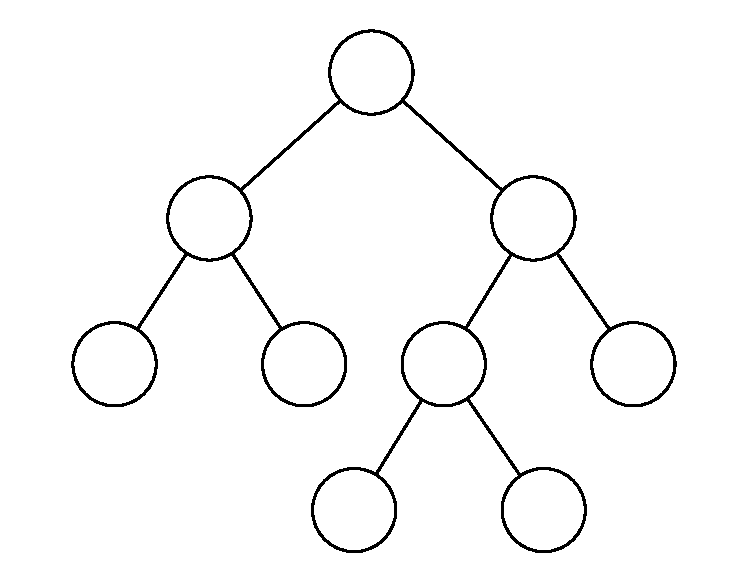
\includegraphics{anal2}
\end{center}

\chapter{Метод классов эквивалентности}

\section{Математические сведения}

\begin{enumerate}
    \item Отношение $R$ на $A$ $R \subset A \times A$
    \item Если $R$ - отношения эквиваленстности:

        \begin{enumerate}
            \item $(a,a) \in R$ - рефлекс
            \item $(a,a') \in R \Rightarrow (a',a) \in R$ - симметричность
            \item $(a,a') \in R, (a', a'') \in R \Rightarrow (a,a'') \in R$ - транзитивность
        \end{enumerate}

    \item Принцип Дирихле P.G.L. Dirichle
\end{enumerate}

\section{Идея метода}

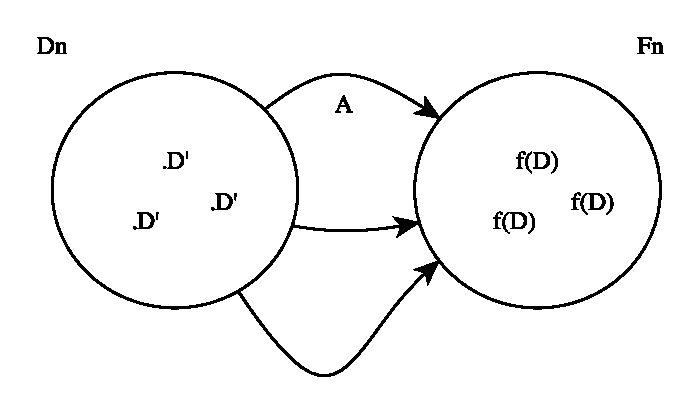
\includegraphics{anal3}

$$
D_n \underset{A}{\to} F_n
$$

$$
f^\vee(n)
$$

$$
\exists D : f(D) = f^\vee + 1
$$

$$
R \text{ на } D_n (D,D') \in R \Leftrightarrow f_A(D) = f_A(D')
$$

$$
f^\vee, f^\wedge P(f(D) = f_1) = \frac{|D_{f_1}|}{|D_n|}
$$

$$
\overline{f_A}(n) = \sum_k f_k \cdot P(f = f_K)
$$

\subsection{Реализация}

\begin{enumerate}
    \item Равномощное разбиение
    \item Объединение в классы
\end{enumerate}

\section{Сортировка 3х чисел по методу}

\begin{lstlisting}
Sort3(a,b,c) $\leftarrow D_3$
    if a > b
        then a $\substack{\leftarrow}^\rightarrow$ b
    if b > c
        then b $\substack{\leftarrow}^\rightarrow$ c
    if a > b
        then a $\substack{\leftarrow}^\rightarrow$ b
End
\end{lstlisting}

\begin{tabular}{ccccc}
    $a,b,c$  & &           & $f$ & $f^\vee$ \\
    \hline
    1 - min  & & $D_{123}$ & 3   & \\
    2 - midl & & $D_{132}$ & 6   & \\
    3 - max  & $\Rightarrow$ & $D_{213}$ & 6   & $\overline{f} = 7 \frac{1}{2}$\\
             & & $D_{231}$ & 9   & \\
             & & $D_{312}$ & 9   & \\
             & & $D_{321}$ & 12  & \\
\end{tabular}

\subsection{Модификация}

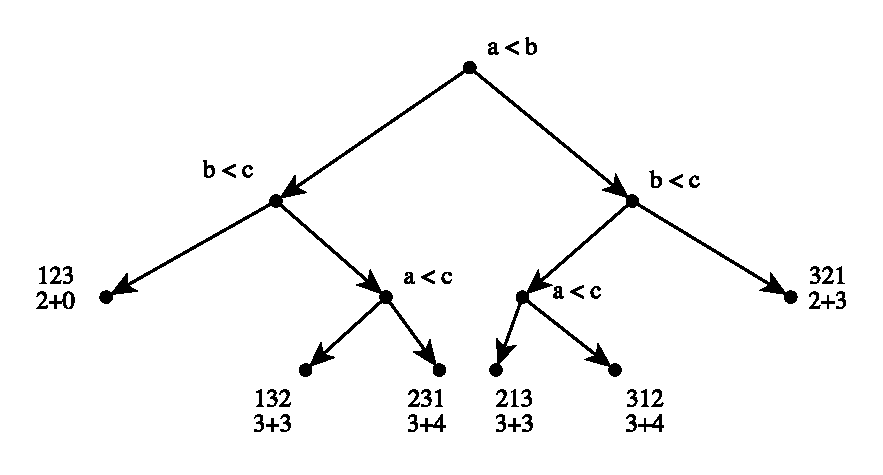
\includegraphics{anal4}

\begin{tabular}{ccc}
              & $f^\vee$ & \\
    \hline
    $D_{123}$ & 2        & \\
    $D_{132}$ & 6        & \\
    $D_{213}$ & 6        & $\overline{f} = 5 \frac{1}{2}$\\
    $D_{231}$ & 7        & \\
    $D_{312}$ & 7        & \\
    $D_{321}$ & 5        & \\
\end{tabular}

\section{Анализ max}

\begin{lstlisting}
M $\leftarrow$ A[1]
for j $\leftarrow$ 2 to n
    if M < A[j]
        then M $\leftarrow$ A[j]
\end{lstlisting}

$$
D_4 \to n = 4
$$

\begin{tabular}{ccc}
    1 - min  & 2 1 3 4 qqqq\\
    2 - min2 & 2 1 4 3 \\
    3 - max2 & 2 3 1 4 \\
    4 - max  & 2 3 4 1 \\
\end{tabular}

$$
g_n(x) = x^{\overline{n}}
$$

$$
g_4(x) = x(x+1)(x+2)(x+3)
$$

$$
g_4(1) = 24
$$

$$
g_4(x) = 1 \cdot x^4 + 6 \cdot x^3 + 11 \cdot x^2 + 6 \cdot x
$$

$$
S_n^k
$$

\end{document}
